
\section{Implementation}
\label{sec:Implementation}

\subsection{Komponenten}
\label{impl:Komponenten}

\subsection{QGIS Plugin}
\label{impl:QGIS Plugin}
TODO

\subsection{PlazaRoute Container}
\label{impl:PlazaRoute Container}
TODO

\subsubsection{Plaza Vorverarbeitung}
\label{impl:Plaza Vorverarbeitung}
TODO

\subsubsection{Plaza Routing}
\label{impl:Plaza Routing}
In den folgenden Unterkapitel wird die Umsetzung der Plaza Routing Architektur, welche im Kapitel \ref{architektur:Plaza Routing} definiert ist, erläutert. 

\paragraph{api}\label{impl:Plaza Routing api}~\\
In diesem Kapitel wird auf die Umsetzung der api-Schicht in Abbildung \ref{fig:package_diagram_plaza_routing} Bezug genommen.

TODO Flask Setup beschreiben

\paragraph{Zusammenspiel und Verantwortlichkeit}\label{impl:Plaza Routing Zusammenspielund Verantwortlichkeit}~\\
In Abbildung \ref{fig:sequence_diagram_plaza_routing_overview} sind die Interaktionen zwischen den Komponenten in einem Sequenz-Diagramm aufgeschlüsselt. Dabei wurde zur Wahrung der Übersichtlichkeit das Holen aller möglichen Routen in Unter-Squenz-Diagram in Abbildung \ref{fig:sequence_diagram_plaza_routing_route_combs} ausgelagert. Dabei geht es nicht primär um die Logik die dahinter liegt, sondern um die Verantwortlichkeiten der Services. Wann sie ins Spiel kommen und für was sie benötigt werden, ist so gut ersichtlich.

\begin{figure}[ht]
    \centering
    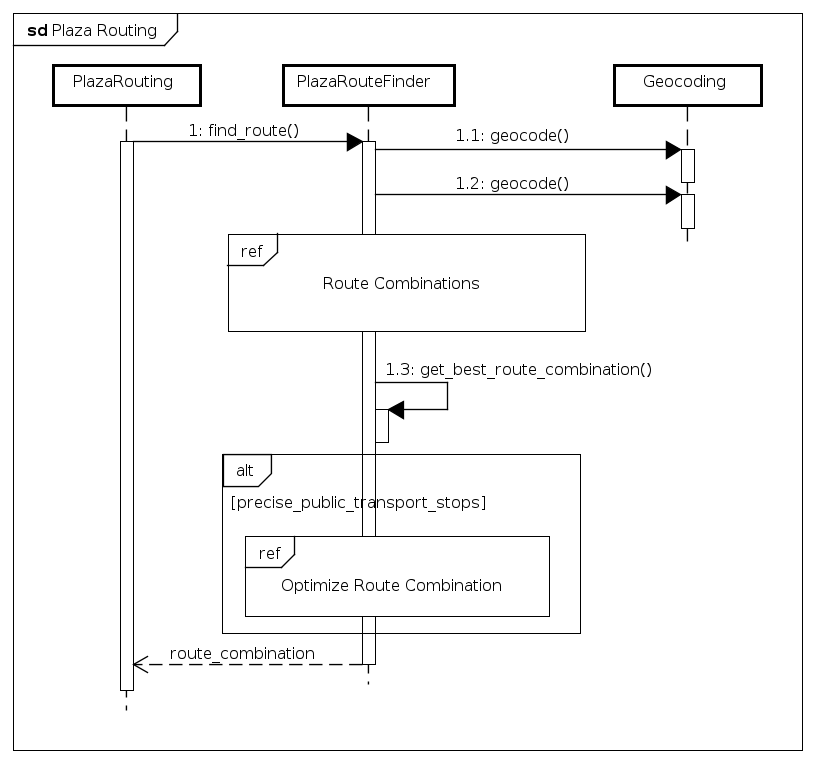
\includegraphics[width=0.7\linewidth]{projectdoc/img/sequence_diagram_plaza_routing_overview}
    \caption[Plaza Routing Sequenz-Diagramm Übersich]{Plaza Routing Sequenz-Diagramm Übersicht}
    \label{fig:sequence_diagram_plaza_routing_overview}
\end{figure}

\begin{figure}[ht]
    \centering
    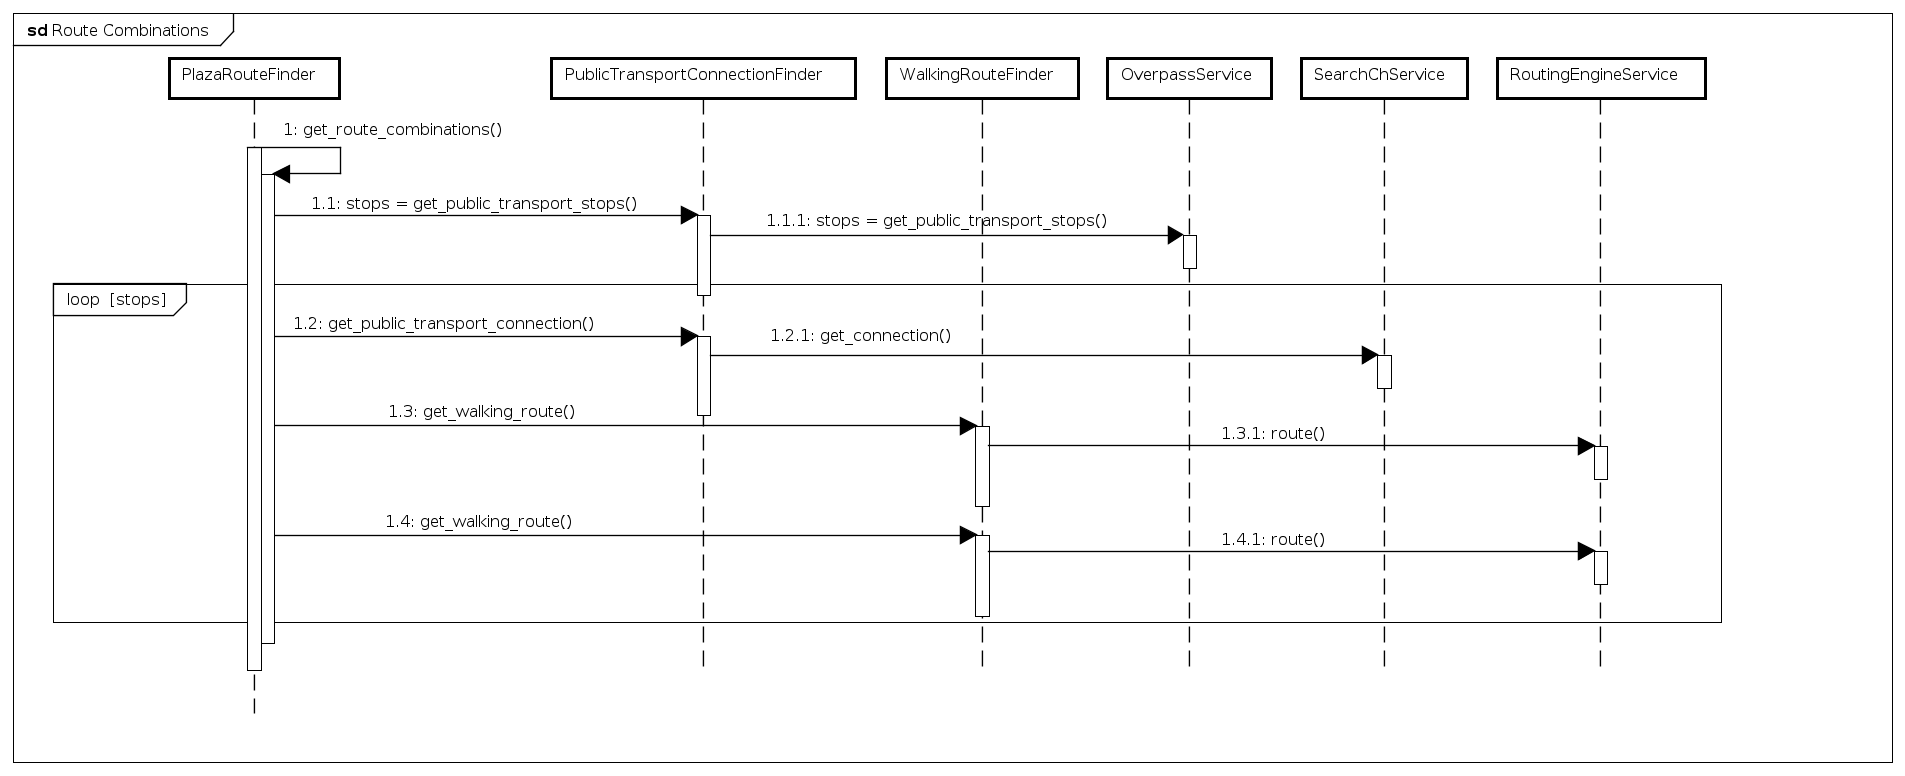
\includegraphics[width=1\linewidth]{projectdoc/img/sequence_diagram_plaza_routing_route_comb}
    \caption[Plaza Routing Sequenz-Diagramm Route Combinations]{Plaza Routing Sequenz-Diagramm Route Combinations}
    \label{fig:sequence_diagram_plaza_routing_route_combs}
\end{figure}


Herauszuheben ist, dass \emph{PublicTransportRouteFinder} in Schritt 6 zuerst die ÖV-Haltestellen in der Nähe eruiert (siehe \ref{impl:Plaza Routing ÖV-Haltestellen eruieren}) und für jede Haltestelle die ÖV-Verbindung über \emph{SearchChService} iterativ in Schritt 7 von search.ch \cite{search_ch_route_api} bezieht.

\paragraph{ÖV-Haltestellen eruieren}\label{impl:Plaza Routing ÖV-Haltestellen eruieren}~\\
ÖV-Haltestellen werden mit Overpass \cite{wiki:overpass} aus \ac{OSM} bezogen. Dabei wird um den aktuellen Standort eine \gls{BoundingBox} gezogen. Die Bounding Box ist konfigurierbar und entspricht einer zumutbaren Laufdistanz. In dieser Fläche werden Nodes und Relationen mit Tags, welche ÖV-Haltestellen identifizieren (\emph{''public\_transport''=''stop\_position''}, \emph{''type''=''public\_transport''} etc.), gefiltert und die \emph{uic\_ref} zurückgegeben.

\paragraph{Beste Route eruieren}\label{impl:Plaza Routing Beste Route eruieren}~\\
TODO mit Sequenzdiagram

\paragraph{inkonsistentes ÖV-Mapping}\label{impl:Plaza Routing inkonsistentes ÖV-Mapping}~\\
Mit Hilfe von Overpass \cite{wiki:overpass} wird für eine ÖV-Verbindung die korrekte Koordinate der Einstiegs- und der letzten Endhaltestelle geholt. Search.ch \cite{search_ch_route_api} liefert in ÖV-Verbindung für zwei gegenüberliegenden Haltestelle (je eine für jede Fahrrichtung) eine Koordinate zurück, welche beispielsweise direkt auf der Hauptstrasse liegen kann. Dies ist für ein Fussgänger-Routing nicht optimal.
Da ÖV-Stationen und -Linien in \ac{OSM} nicht konsistent gemappt sind, wird das Recovery Blocks Pattern \cite{fault_tolerant_software} angewendet, um dem User so gut wie möglich ein genaues Resultat zu liefern.
%TODO Problematik mit OSM-Daten und Recovery-Block Pattern in Implementation verschieben
